\documentclass[a4paper,10pt]{article}
\input{/home/frr/UFSC/Pagina/Dropbox/Modelos/Modelo_prova_latex/estilo_prova.tex}

\begin{document}


\professor{Fábio Rodrigues de la Rocha}
\turma{06655}
\codigodisciplina{ARA7546}
\disciplina{Circuitos Digitais}
\data{24/03/2014}
\hlimite{20:20}
\listaexercicios{6}

\begin{center}
\large{\fbox{\mbox{Contadores}}}
\end{center}


\questao{Utilizando flip-flops J-K mostre como construir um contador crescente assíncrono de 4 bits.}

\questao{Diferencie contador síncrono de contador assíncrono.}

\questao{Modifique o contador da primeira questão para permitir uma contagem crescente e decrescente, baseado numa linha \texttt{MODO\_OPERACAO}.}

\questao{Construa um contador de números não naturais capaz de contar a seqüência 5,3,4,0,1,2, ou seja. O Contador inicia no número 5 e a cada pulso de clock
muda seu valor para o próximo elemento da seqüência. Quando a seqüência chega ao fim o contador retorna ao número 5. Mostre as equações para os Flip Flops JK e
desenhe o circuito eletrônico e as ligações necessárias. OBS: Talvez você nao precise de todos os FF da figura.}

\begin{figure}[H]
 \centering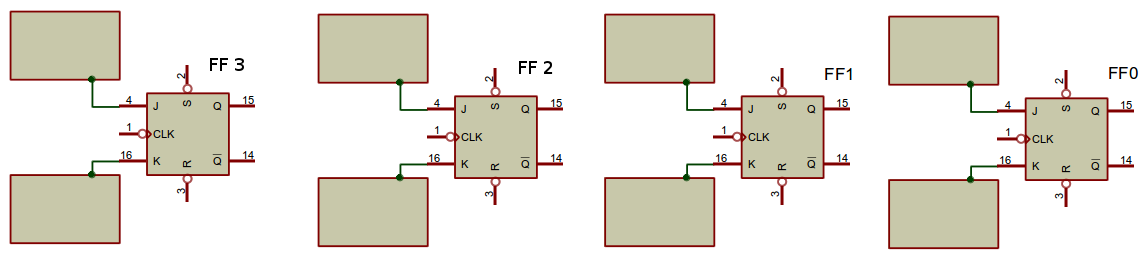
\includegraphics[width=0.6\textwidth]{nao_naturais}
\end{figure}


\questao{Construa um contador síncrono de 4 bits (usando FF J-K) para contar a sequencia não natural 0, 12, 15, 2, 3, 4, 9, 14, 7, 8, 11, 5.}


\begin{figure}[H]
 \centering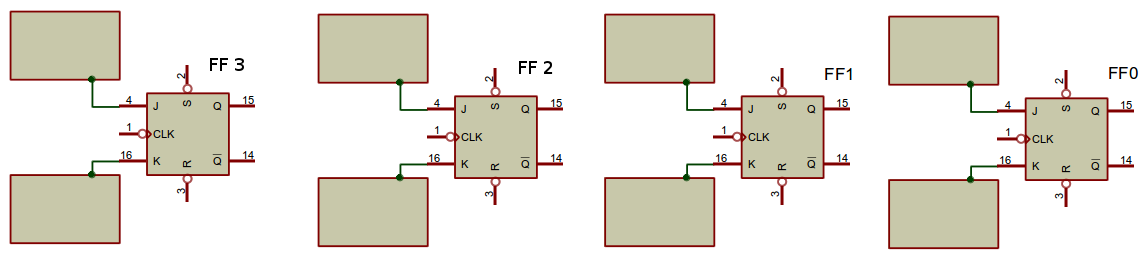
\includegraphics[width=0.6\textwidth]{nao_naturais}
\end{figure}

\questao{Utilizando associações do  CI 7490 mostre como construir um contador que conta até 17 e trava.}

\begin{figure}[H]
 \centering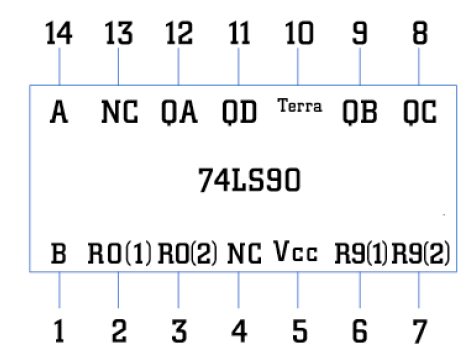
\includegraphics[width=0.2\textwidth]{7490}
\end{figure}

\questao{Utilizando associações do CI 7490 crie um cronômetro que conte horas, minutos e segundos. Assuma que existe disponível um clock base de 1Hz.}

\questao{Utilizando associações do CI 7490 crie um divisor de frequencia por 43.}

\questao{Projete um circuito contador que inicie uma contagem crescente do número 0 e ao atingir o número 21 mude a direção de contagem e conte até 12. Ao atingir
o número 12, ele deve novamente voltar a contar em ordem crescente, mas desta vez até o número 30 quando a contagem pára. Além disso, existe um LED que
inicialmente deve ficar aceso e que quando o contador atinge o valor 15 pela primeira vez deve ser apagado. Quando o contador atinge o valor 15 pela segunda vez,
o LED volta a ficar ligado, permanecendo neste estado. O LED é controlado gerando um sinal ESTADO\_LED para acender ou apagar o LED. Implemente este circuito
utilizando somente Flip-Flops JK (chaveado na borda positiva ou negativa), CI 74193 e portas lógicas se necessário.}



	
\begin{figure}[H]
\begin{minipage}[b]{0.3\textwidth}
\centering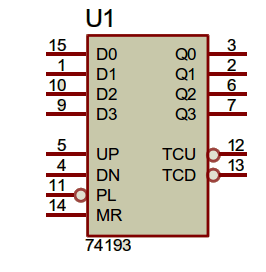
\includegraphics[width=0.6\textwidth]{74193}
\end{minipage}
\hspace{0.5cm}
\begin{minipage}[b]{0.3\textwidth}
\centering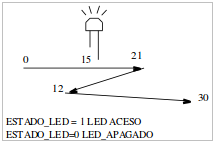
\includegraphics[width=0.6\textwidth]{led}
\end{minipage}
\end{figure}


No CI 74193 (Contador binário) mostrado acima, D0..D3 são entradas, Q0..Q1 são saídas, PL é de (Load em Paralelo), UP/DN é para fazer operação de UP e Down. Os
pinos TCU e TCD são usados para cascateamento. O TCU é usado para sinalizar um Carry e o TCD é usado para sinalizar um “empréstimo”. O pino MR serve para zerar o
contador.

\questao{Uma roda de bicicleta possui um sensor magnético que a cada giro da roda gera um pulso em nível alto. A roda da bicicleta possui aproximadamente 0,30
cm de raio. Construa um dispositivo que mostre em 3 displays de 7 segmentos a distancia percorrida pela bicicleta. O display menos significativo indica dezenas de
metros, o display do meio indica centenas de metros e o display mais significativo indica milhares de metros. Assuma em seus cálculos duas casas depois da vírgula
e o valor de $\pi=3,14$. Utilize CIs contadores 74190.} Você precisará arredondar valores.

\begin{figure}[H]
\begin{minipage}[b]{0.4\textwidth}
\centering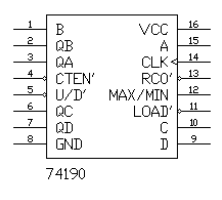
\includegraphics[width=0.6\textwidth]{74190}
\end{minipage}
\hspace{0.5cm}
\begin{minipage}[b]{0.6\textwidth}
\centering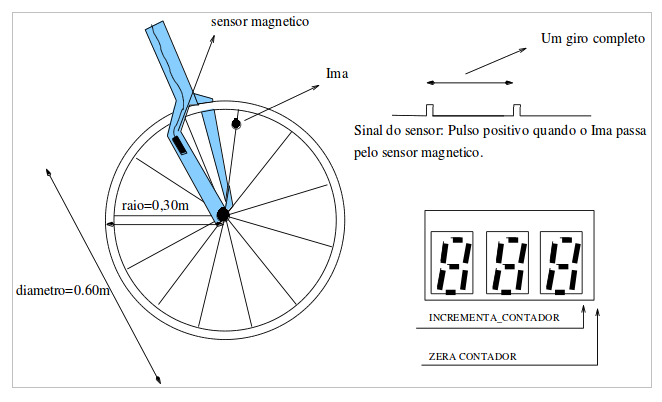
\includegraphics[width=0.6\textwidth]{bicicleta}
\end{minipage}
\end{figure}


\questao{Numa industria existe uma esteira móvel que transporta caixas de 3 tamanhos diferentes. No final da esteira existem 3 sensores óticos (A,
B e C) que servem para determinar a quantidade de caixas de cada tamanho que saem da esteira. Você foi contratado para criar um circuito contador que mostre em 2
dígitos quantas caixas de cada tamanho passaram pela esteira. O sensor funciona por interrupção de um raio de luz. Utilize o CI 7490 (pinagem no final da prova),
decodificadores de 7 segmentos e displays de 7 segmentos. Interprete corretamente a leitura dos sensores óticos e associe os contadores para fornecer os valores
esperados. No exemplo mostrado, quando uma caixa grande passa pelo final da esteira percebemos uma interrupção no raio de luz (sinal em nível baixo entre x e y).}

\begin{figure}[H]
 \centering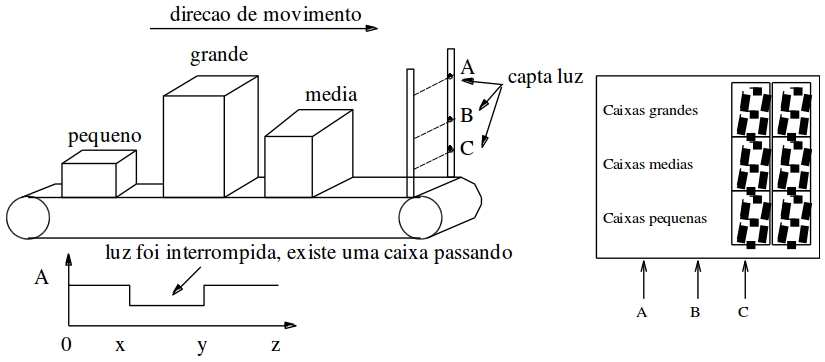
\includegraphics[width=0.6\textwidth]{esteira}
\end{figure}


\end{document}